\section{Background}
%\section{Aikaisempi tutkimus}

\subsection{Power requirements of a sensor}
The sensor system will be in three distinct states. One is sleeping, conserving power as much as possible while car is not moving.
Second state is measuring, when the radio connection is off but electronics are active and gathering data.
Third state is transmitting, when the data is relayed to drive computer in car.

Energy and power consumption are estimated by reviewing a few suitable components and their power requirements. 
Energy management is handled by a specialized integrated circuit (IC), for example LTC3331 \cite{Technology}.

Communication is handled by a Bluetooth-low energy (BLE) module, which contains a general-purpose microcontroller for application flow control.
We use BLE113 {\color{red} refer to datasheet} as an example of such module.

Finally there is an accelerometer which is used for gathering data out of the system, ADXL375 {\color{red} reference to datasheet} is used as an example. ADXL is a low-power digital accelerometer with dynamic range of 200g. Table \ref{power_consumption_table}  summarizes the estimated power requirement of each subsection of system. System level voltage is selected to be 2.5 V, as that is lowest voltage which LTC3331 can supply and allows all devices to function. Lowest possible voltage is selected to reduce the power draw.

\begin{table}[htb]
%% Taulukon teksti
\caption{\label{power_consumption_table} Current and power consumption of system at different activity levels.}
\begin{center}
\fbox{
\begin{tabular}{l l r r}
\textbf{Device}		& \textbf{Sleep} 	& \textbf{Monitoring}	& \textbf{Communicating}\\ \hline
LTC3331			& 0.2 $\mu A$		& 80 $\mu A$ 		& 16 250 $\mu A$ 		\\ \hline
BLE113			& 0.9 $\mu A$ 		& 275 $\mu A$ 		& 26 000 $\mu A$	\\ \hline 
ADXL375			& 0.1 $\mu A$ 		& 140 $\mu A$ 		& 140 $\mu A$		\\ \hline \hline
\textbf{Total power}	& 3   $\mu W$		& 3!! $\mu W$		& 65 375!! $\mu W$	
\end{tabular}
}
\end{center}
\end{table}

Power consumption grows by two orders of magnitude when the activity is stepped up to next level. Therefore it's important to keep the system in sleep whenever possible, for example when the car is parked and wake up only periodically to check if movement has started. Monitoring starts once car is moving, and device will send brief pulses over the radio link when necessary.

Battery manager power draw is estimated by calculating required power to supply the rest of the circuit at 80 \% efficiency.

\subsection{Powering the sensor}
Traditionally wireless sensors have been powered with either primary or rechargable batteries. These systems need service at regular intervals to change or recharge the batteries. In applications where battery cannot be reached, battery lifetime often limits the lifetime of whole system. Alternative approach has been to use generators, such as fuel cells or even radioactive power sources. These systems often have a poor power density and decreasing efficiency when scaled down to small size \cite{Knight2008}. 

This work explores ways to utilise energy present in tyre to power the sensor itself. A single tyre can waste as much as 500 W of power at high speeds {\color{red} source}, so harvesting even 1/100 000ths of wasted power would be enough for a well designed low-power sensor and transmitter.

There are many different energy harvesting solutions which use fundamentally different physical principles and energy sources, such as thermal, solar, radio waves and mechanical. {\color{red} source}. As the energy harvester is inside tyre, solar harvesting is unfeasible. Radio wave harvesting methods rely on external radio transmissions for gathering power. As the device should work regardless of external environment, these methods are not suited for application. Thermal methods require significant temperature gradients {\color{red} source}, but previous work shows that car tire can reach only ambient plus few tens of \degree C {\color{red} source}. Therefore thermal methods would be ineffective. 

Mechanical energy harvesting is a natural choice, as there is abundant amount of mechanical energy available as accelerations, vibrations and centrifugal{\color{red}?} force available inside the tyre. There are various different approaches for harvesting mechanical energy, including piezoelectronic, electrostatic, electromagnetic and microelectromechanical systems (MEMS) {\color{red} source}. To select optimal method for energy harvesting, more information about the characteristics of mechanical energy is required.

{\color{yellow} refer to \cite[p.10]{Kubba2014}}

The power requirements of system create additional constraints on energy harvesting method, as the energy harvester must be able to supply enough energy and power to system.

\subsection{Environment inside tire}
The energy harvester will be placed inside the tyre. Previous studies in department have shown
that the tyre will experience acceleration in all three axes {\color{red} source}. Tangential and centripetal accelerations are dominant,
they can reach amplitudes of up to 150g in text fixture. 

In addition, literature suggests shock survival of up to {\color{red}n hundered g} is required for reliability. {\color{red} source}

Temperature inside of the tire will reach equilliberium in ambient + 5-10 \degree C, so operation temperature should be
in range of -40 to + 75 \degree C to have some safety margin on top of usual Finnish ambient conditions.

As cars move from place to place, any energy source from environment outside the tire cannot be relied upon. 
{\color{blue} Merge with Acceleration and vibration characteristics?}

\subsection{Acceleration and vibration characteristics of tyre}
Previous work by {\color{red}[Niskanen, Tuononen]} was used to as a basis for analysis of characteristics of acceleration inside tire. Raw data was used to gather minimum and maximum values of acceleration as well as frequency components inside tire. Data was gathered at 20 km/h, 60 km/h and 80 km/h speeds. 

Figures {\color{red}[Kuva 1, Kuva2 ]} are time domain representations of the acceleration along 3 axes {\color{red}Lis\"a\"a kuva jossa akselien suunnat}. First figure shows 10 rotations if tyre, contact with drum is clearly visible as a sudden shock. Second figure is a zoom into one rotation.

Frequency domain representations were calculated in Matlab. There are two main contributors to base frequencies: first is the rotational frequency of tyre itself and second is the impact when the tyre deforms as it contacts the drum.. There is clearly visible series of frequency components spaced at the rotational frequency of tyre as well as shock harmonics at upper frequencies. 

\begin{figure}[htb]
\begin{center}
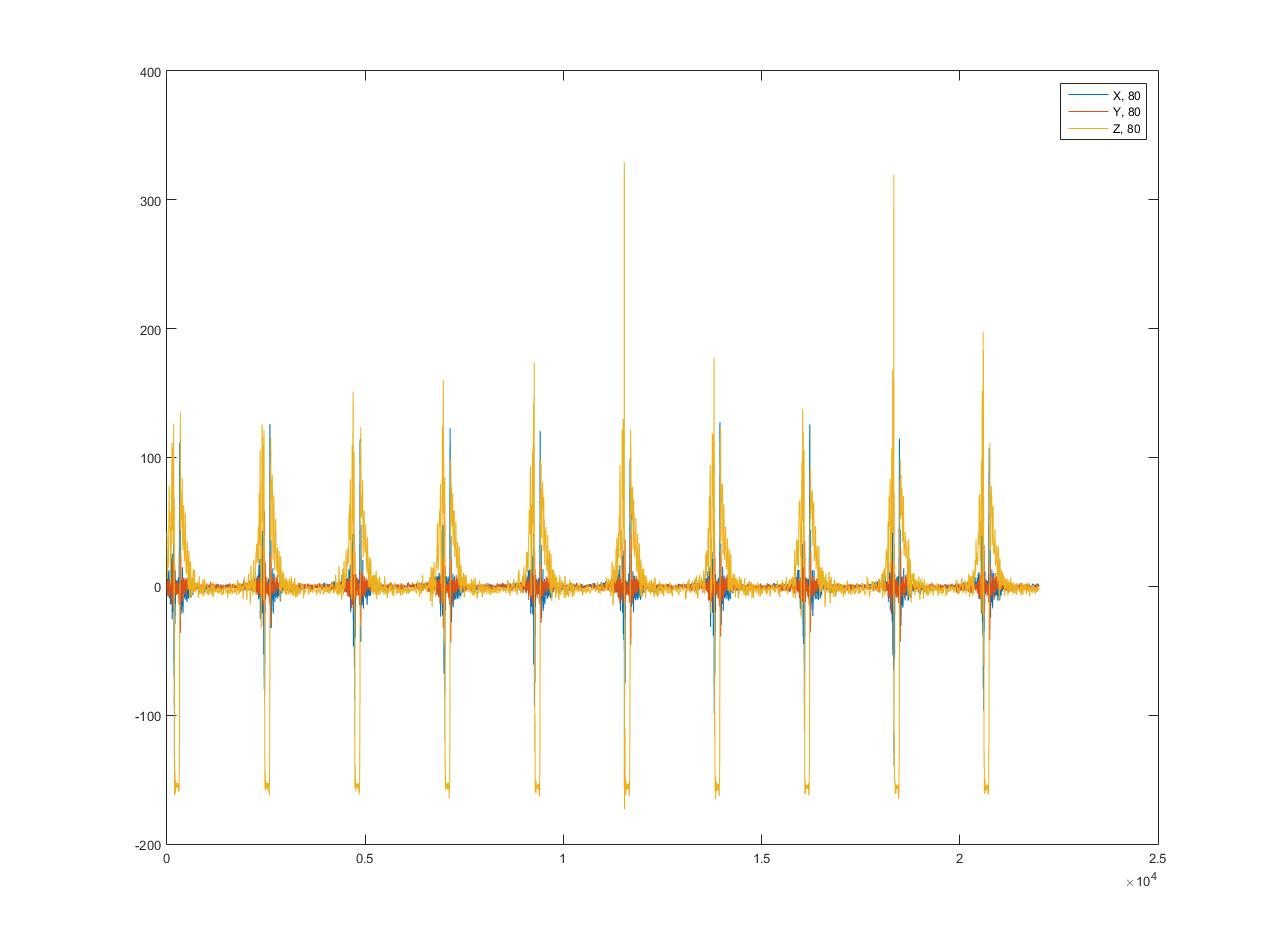
\includegraphics[height=8cm]{images/80kmh_timedomain}
\end{center}
\caption{Kuvateksti, jossa on liitteen numerointi {\color{red}lahdeviittaus}}
\label{liitekuva}
\end{figure}

\begin{figure}[htb]
\begin{center}
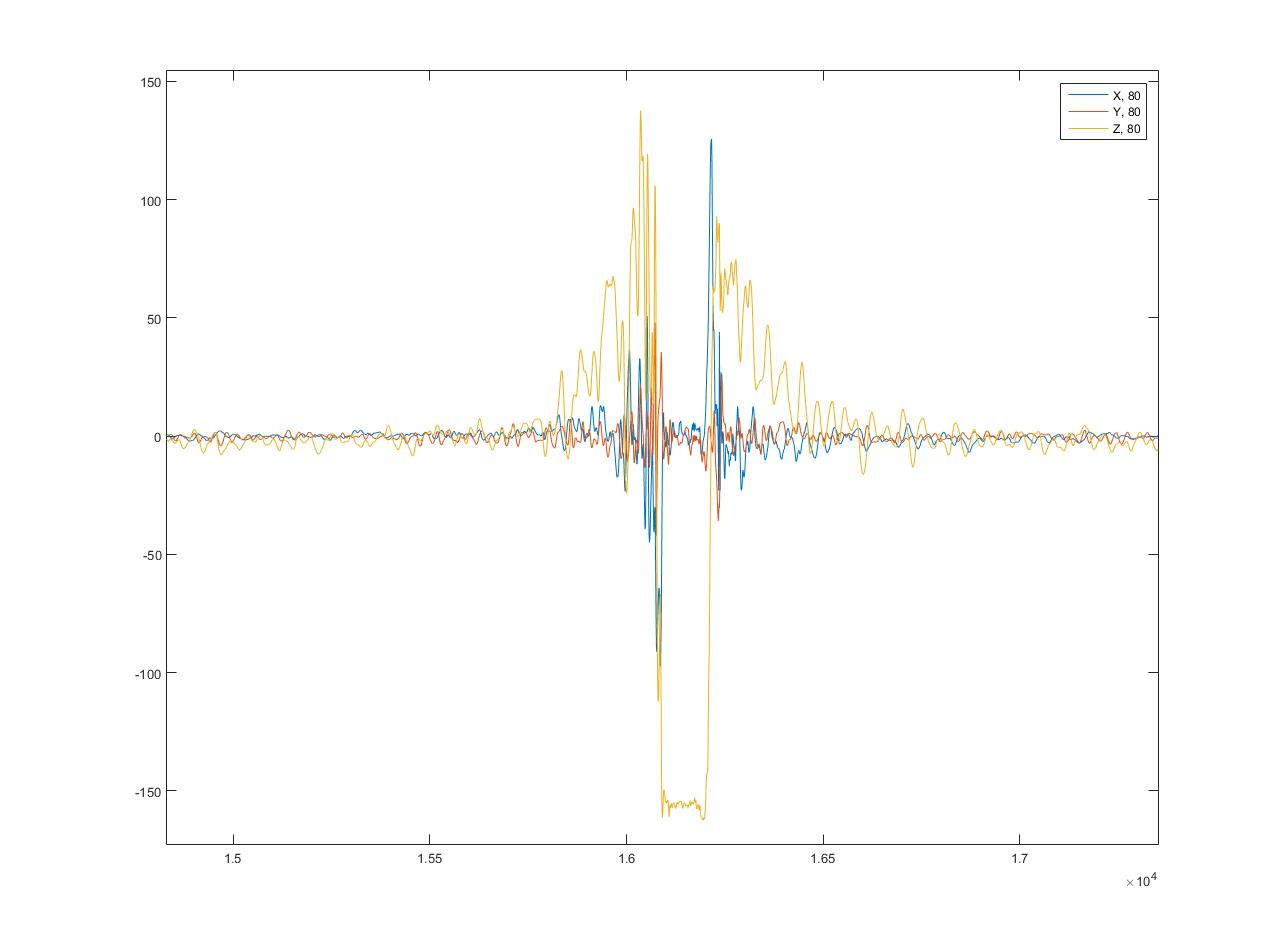
\includegraphics[height=8cm]{images/80kmh_timedomain_onerotation}
\end{center}
\caption{Kuvateksti, jossa on liitteen numerointi {\color{red}l\"ahdeviittaus}}
\label{liitekuva}
\end{figure}

\begin{figure}[htb]
\begin{center}
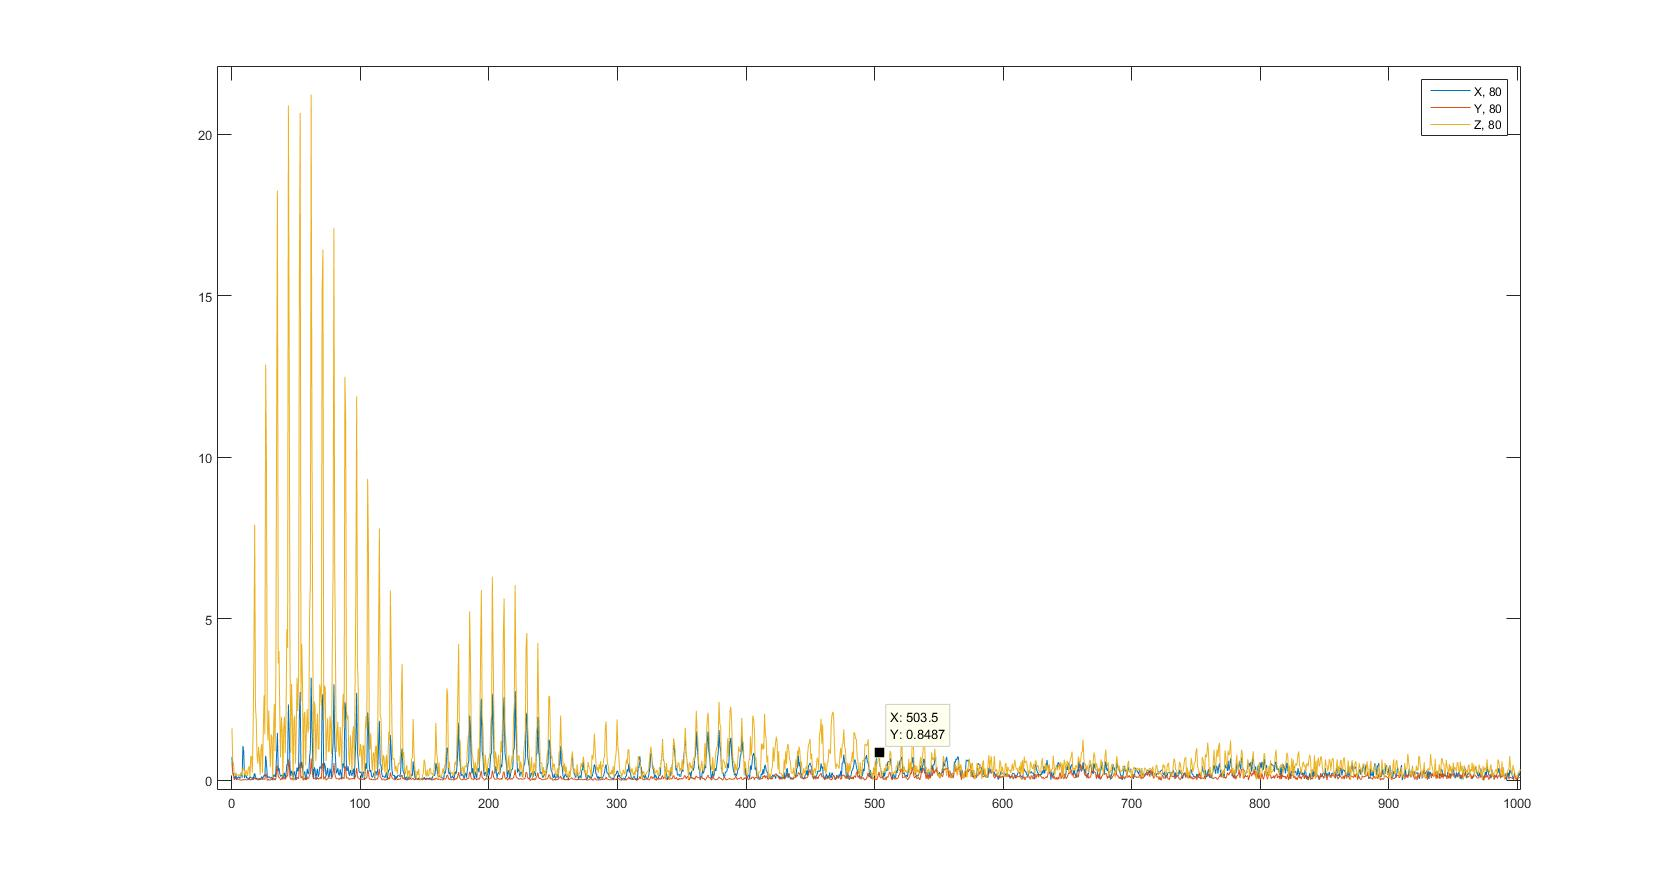
\includegraphics[height=8cm]{images/FFT-80}
\end{center}
\caption{Kuvateksti, jossa on liitteen numerointi {\color{red}l\"ahdeviittaus}}
\label{liitekuva}
\end{figure}

\begin{figure}[htb]
\begin{center}
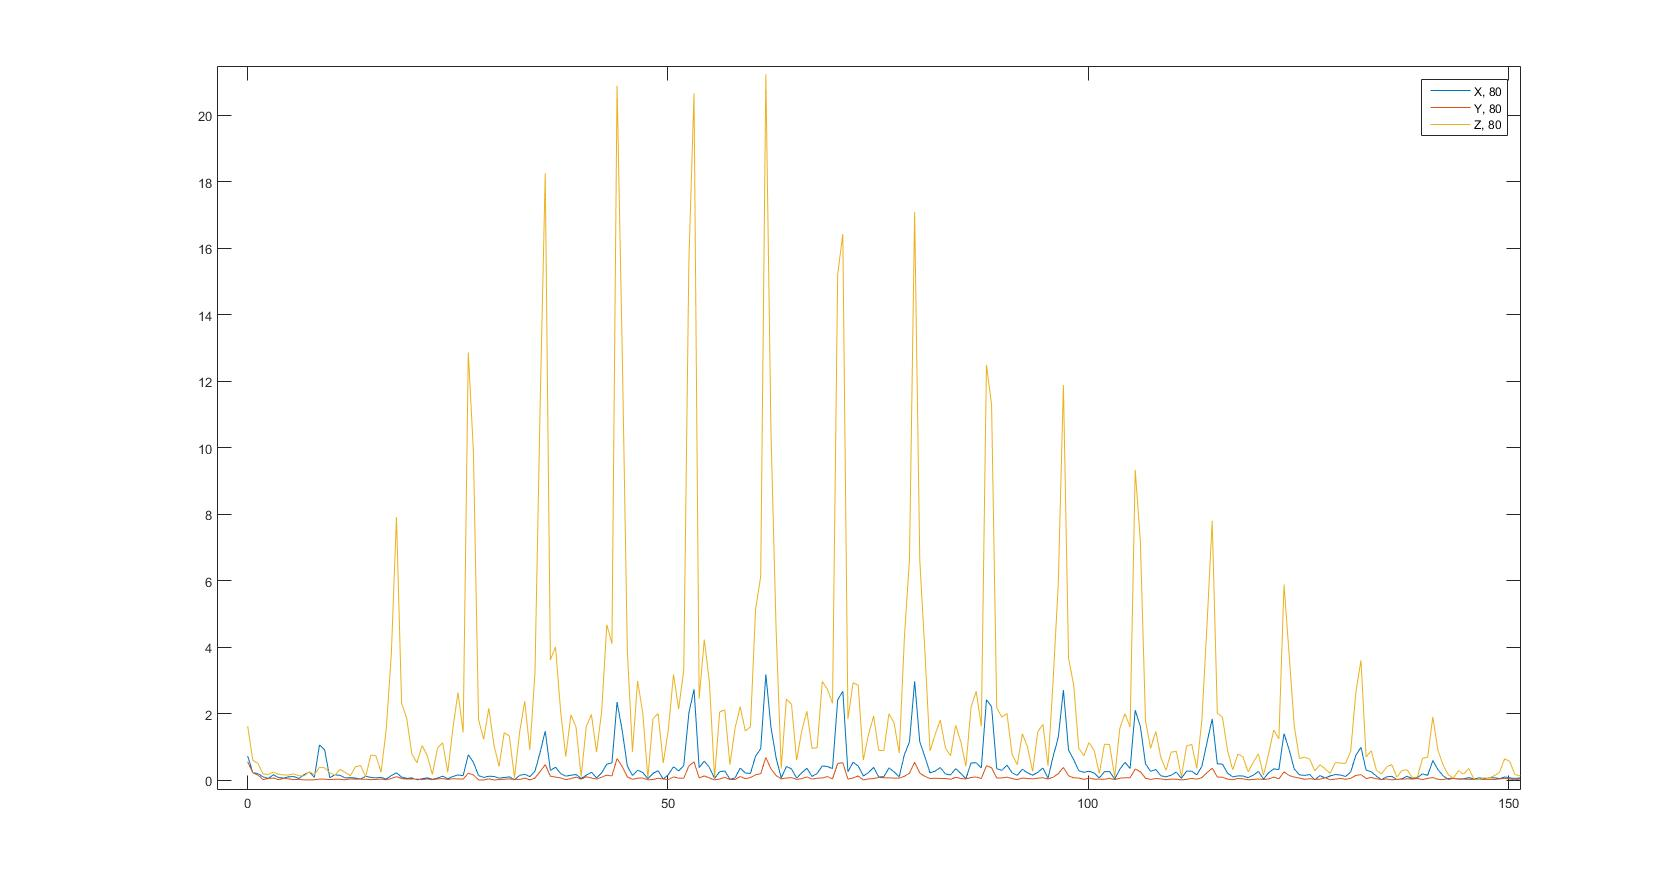
\includegraphics[height=8cm]{images/FFT-80-zoom}
\end{center}
\caption{Kuvateksti, jossa on liitteen numerointi {\color{red}l\"ahdeviittaus}}
\label{liitekuva}
\end{figure}

It's important to notice that the sensor used was piezoelectric, which forms a highpass filter as the operation is based on charge between layers. This charge dissipates over time, so the steady-state centripetal acceleration reads as zero. There is a constant acceleration on the device caused by rotational movement by the tire. 
